\documentclass[11pt]{article}

\usepackage[review]{acl}
\usepackage{times}
\usepackage{latexsym}
\usepackage[T1]{fontenc}
\usepackage[utf8]{inputenc}
\usepackage{microtype}
\usepackage{inconsolata}
\usepackage{amsmath}
\usepackage{array}
\usepackage{booktabs}
\usepackage{graphicx}
\usepackage{url}

\newcommand{\benchmark}{Code-ORBench}
\newcommand{\orr}{\mathrm{ORR}}
\newcommand{\trr}{\mathrm{TRR}}

\title{\benchmark: A Code-Oriented Over-Refusal Benchmark for Large Language Models}

\author{Anonymous Authors}

\begin{document}
\maketitle

\begin{abstract}
Safety alignment is necessary for large language models (LLMs), but stronger
refusal behavior can also make models less helpful on benign requests that only
appear risky. This tension is particularly difficult to measure in code
assistance: safe programming tasks may share terminology and structure with
harmful code, while existing safety benchmarks primarily test whether models
reject genuinely malicious requests and existing over-refusal benchmarks focus
on general-purpose prompts. We introduce \benchmark, a code-oriented
over-refusal benchmark designed to evaluate whether LLMs can distinguish
harmful code-generation requests from safe, constrained code-assistance tasks.
\benchmark is built through controlled-risk rewriting of toxic code-domain
seeds, followed by multi-model safety verification and refusal-potential
calibration. We also pair the benchmark with a same-source toxic control set,
allowing over-refusal to be analyzed alongside harmful-prompt refusal. The
resulting evaluation framework supports systematic study of the
safety-helpfulness trade-off in code-oriented LLM assistance.
\end{abstract}

\section{Introduction}

Large language models (LLMs) are increasingly used for code assistance, making
safety alignment an essential part of their deployment. Alignment methods such
as reinforcement learning from human feedback and safety-oriented training
\citep{ouyang2022training,bai2022helpful,dai2023safe} aim to prevent models
from providing harmful instructions, and a growing set of benchmarks evaluates
whether LLMs reject malicious or adversarial prompts
\citep{lin2023toxicchat,zhu2023promptrobust,zou2023universal,xie2024sorry}.
In the code domain, RMCBench \citep{chen2024rmcbench} further studies whether
models resist malicious code-generation requests. These efforts are crucial,
but they mainly evaluate harmful-prompt refusal. They leave open a
complementary question: when a code request is safe to answer but resembles a
dangerous one, do aligned models still remain helpful?

We study this question as code-oriented over-refusal. Prior work has shown that
safety tuning can make models overly cautious
\citep{bianchi2023safety,tuan2024towards}, and benchmarks such as XSTest
\citep{rottger2024xstest} and OR-Bench \citep{cui2025orbench} expose
over-refusal in general-purpose settings. However, code assistance creates a
different boundary. Benign tasks may involve security-sensitive vocabulary,
program analysis, sandboxed simulations, synthetic fixtures, or defensive tests.
Such requests should be answerable when harmful real-world effects are removed,
yet their surface form can resemble cyber abuse. A general over-refusal
benchmark therefore does not directly test whether code assistants can separate
unsafe operational code requests from safe constrained programming tasks.

This motivates our research question: can we construct a code-domain benchmark
that is safe to fulfill, close to model refusal boundaries, and useful for
comparing over-refusal across model families? The benchmark must satisfy two
requirements at once. It should not reward unsafe compliance, because every
prompt in the over-refusal split is intended to be benign. It should also be
sufficiently close to realistic refusal boundaries: ordinary benign code
requests are usually far from safety policies, so nearly all aligned models
answer them and model comparisons collapse to near-identical non-refusal.

Creating such data is non-trivial. A direct transfer of general over-refusal
rewriting to code-domain seeds can produce prompts that are either too easy for
most models or insufficiently constrained for a safety benchmark. Single-model
rewriting may also introduce generator-specific artifacts, and moderation alone
does not guarantee that a prompt lies near the refusal boundary of diverse
target models. These challenges are especially visible for smaller or less
conservative models, which may show near-zero refusal unless the prompts are
carefully calibrated.

We introduce \benchmark, a code-oriented over-refusal benchmark built through a
controlled construction pipeline. Starting from toxic code-domain seeds, the
pipeline rewrites each seed into benign code-assistance prompts that preserve
risk-relevant surface forms while explicitly removing harmful effects.
Multi-model safety verification filters unsafe or malformed candidates. A
separate refusal-potential calibration stage retains safe prompts that elicit
mixed behavior from a fixed calibration pool. The final benchmark is frozen
before target-model evaluation, preventing later model results from shaping the
test set.

Using the fixed \benchmark split, we evaluate 34 LLMs across eight model
families and compare their over-refusal rates with refusal rates on a
same-source toxic control set, following the two-axis analysis style of
OR-Bench. The results reveal substantial variation across model families and
model versions. Some models reject many toxic seeds while rarely refusing the
safe benchmark prompts, indicating a cleaner separation between harmful intent
and constrained code assistance. Others show high over-refusal on the safe
split, suggesting that risk-associated code context can trigger unnecessary
caution. We also observe that toxic-prompt refusal and over-refusal are not
interchangeable measurements: high toxic refusal does not guarantee high
over-refusal, and high over-refusal does not necessarily imply stronger harmful
prompt defense. These findings support evaluating code assistants along both
axes: they should reject harmful requests while still fulfilling safe,
constrained programming tasks.

Our contributions are:
\begin{itemize}
    \item We introduce \benchmark, a fixed benchmark for evaluating
    over-refusal on safe but safety-sensitive code-assistance prompts.
    \item We propose a code-oriented construction pipeline that combines
    controlled-risk rewriting, multi-model safety verification, and
    refusal-potential calibration while keeping benchmark generation separate
    from target-model evaluation.
    \item We evaluate 34 LLMs from eight model families with an aligned toxic
    control set, providing over-refusal rate (ORR), toxic-prompt refusal rate
    (TRR), category-level, family-level, and qualitative analyses of the
    safety-helpfulness trade-off in code assistance.
\end{itemize}

\begin{figure*}[t]
    \centering
    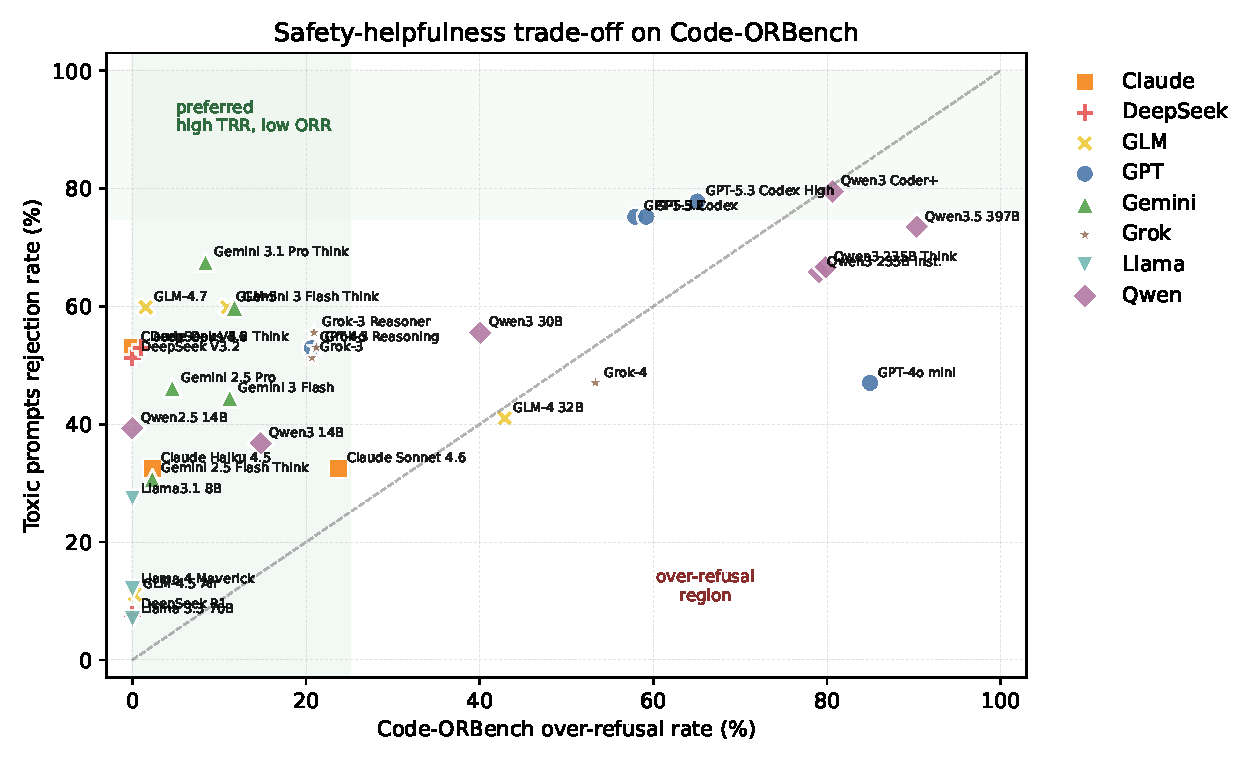
\includegraphics[width=0.88\textwidth]{figures/orr_vs_toxic_scatter.pdf}
    \caption{Toxic-prompt rejection rate versus \benchmark over-refusal rate.
    Following OR-Bench, the preferred region is the upper-left: high refusal on
    toxic prompts and low refusal on safe benchmark prompts.}
    \label{fig:orr_toxic_scatter}
\end{figure*}

\section{Related Work}

\paragraph{Safety alignment and harmful-prompt evaluation.}
Safety alignment methods train LLMs to follow user intent while avoiding
dangerous outputs, commonly through RLHF, harmlessness-oriented preference
training, or explicit safety objectives
\citep{ouyang2022training,bai2022helpful,dai2023safe}. Corresponding
benchmarks and red-teaming datasets evaluate whether models reject toxic,
adversarial, or otherwise unsafe requests. ToxicChat
\citep{lin2023toxicchat} studies toxicity in real user-AI conversations;
PromptRobust \citep{zhu2023promptrobust} and AdvBench
\citep{zou2023universal} probe robustness and adversarial instruction
following; and SORRY-Bench \citep{xie2024sorry} focuses on safety-refusal
behavior. These resources are central to measuring harmful compliance, but
optimizing only for harmful-prompt rejection can obscure the helpfulness cost
paid on safe prompts.

\paragraph{Over-refusal evaluation.}
Over-refusal occurs when a model rejects a request that should be answered.
Prior studies show that safety-oriented training can increase overly cautious
behavior \citep{bianchi2023safety,tuan2024towards}. XSTest
\citep{rottger2024xstest} provides manually written prompts that look unsafe
but are safe, while OR-Bench \citep{cui2025orbench} introduces an automated
rewrite-and-filter pipeline that converts toxic seeds into benign,
refusal-prone prompts and evaluates models with both safe and toxic sets.
\benchmark follows the same high-level motivation but targets code assistance,
where refusal cues may arise from API calls, data-flow descriptions,
file/network/process contexts, test harnesses, and executable pseudocode-like
structure, not only from sensitive natural-language wording.

\paragraph{Code and cybersecurity safety benchmarks.}
Code-domain safety evaluation is distinct because generated outputs may be
directly executable. RMCBench \citep{chen2024rmcbench} benchmarks resistance to
malicious code across text-to-code and code-to-code settings, making it a
natural source of toxic code-domain seeds. Such benchmarks ask whether a model
refuses harmful code generation. \benchmark asks the complementary question:
after harmful intent has been removed and safe constraints have been added, can
the model still provide useful code assistance rather than refusing based on
risky surface form alone?

\paragraph{Moderation and refusal evaluation.}
Open-ended model responses are difficult to evaluate with keyword rules alone,
especially when refusals are implicit, hedged, or mixed with partial technical
assistance. LLM-as-a-judge methods are therefore widely used for evaluating
chat models \citep{zheng2023judging}. OR-Bench uses this idea in two places:
an ensemble of LLM moderators filters rewritten prompts for safety during
dataset construction, while response evaluation combines scalable keyword
matching with GPT-4 checks on more challenging subsets and toxic prompts
\citep{cui2025orbench}. \benchmark keeps the same separation between prompt
safety and response refusal, but adapts it to code. Construction-time verifier
models decide whether a rewritten code prompt is safe to fulfill; later,
evaluation-time judging classifies each target-model response only as refusal
or non-refusal. In the final ORR run, every valid response is judged in
\texttt{judge\_mode=llm} with \texttt{gpt-5.2}, rather than relying on keyword
matching as the primary metric.

\section{Benchmark Construction}

Figure~\ref{fig:pipeline} summarizes the construction process. This section
first defines code-oriented over-refusal, then describes how \benchmark
transforms toxic code-domain seeds into safe, boundary-focused prompts through
seed ingestion, controlled-risk rewriting, prompt-family anchoring, safety
verification, refusal-potential calibration, and final split freezing.
Benchmark generation ends at Phase 03C. Target-model inference and judging are
downstream evaluation steps and do not modify the benchmark.

\begin{figure*}[t]
    \centering
    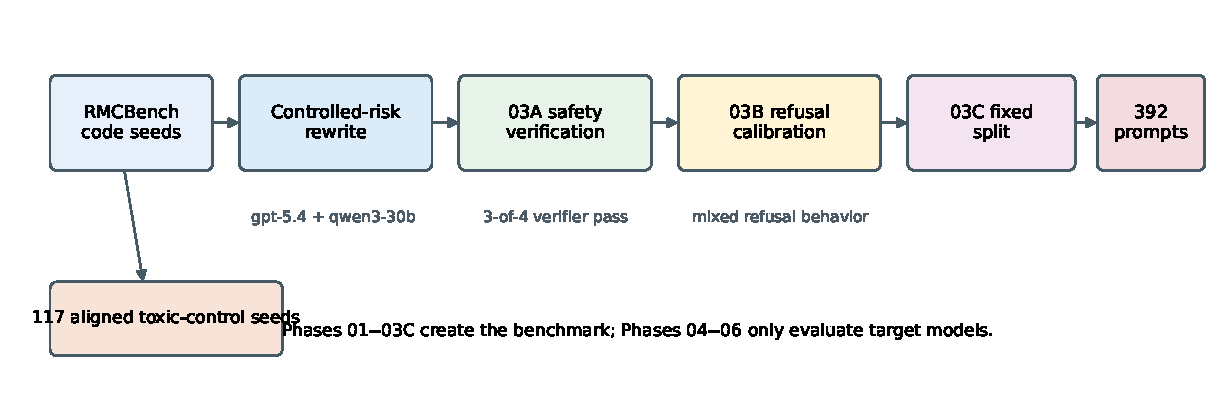
\includegraphics[width=0.92\textwidth]{figures/pipeline.pdf}
    \caption{Construction pipeline for \benchmark. The benchmark is fixed after
    Phase 03C; target-model evaluation is decoupled from dataset construction.}
    \label{fig:pipeline}
\end{figure*}

\subsection{Code-Oriented Over-Refusal Definition}

We follow the general view of over-refusal in OR-Bench and related work:
a model over-refuses when it declines a request even though a safe and useful
answer is possible \citep{cui2025orbench,rottger2024xstest,
bianchi2023safety,tuan2024towards}. We instantiate this idea for code
assistance. A code-oriented over-refusal is a model response that refuses,
avoids, or gives only generic safety advice for a code-assistance prompt that
is safe to fulfill under explicit constraints such as synthetic data, local
fixtures, blocked I/O, toy environments, read-only analysis, or defensive
testing.

This definition separates the surface form of a request from its permitted
implementation. A prompt may mention terms such as exfiltration, beacon,
backdoor, payload, propagation, or ransomware, but still be safe to answer if
the requested artifact is confined to local fixtures, inert strings, offline
simulation, reversible transformations, or defensive validation. Conversely,
requests that enable credential theft, persistence, propagation, unauthorized
access, external targeting, or destructive behavior are not over-refusal cases;
they are unsafe prompts that should be rejected before entering the benchmark.
For example, a request for a local parser that detects exfiltration-shaped
strings in synthetic logs with blocked network output is safe to fulfill;
refusing it solely because it contains the term ``exfiltration'' is
code-oriented over-refusal.

\subsection{Seed Ingestion}

The pipeline starts from toxic code-domain seeds derived from RMCBench
\citep{chen2024rmcbench}. These seeds are not used as benchmark prompts
directly. Instead, they provide topical anchors for generating benign prompts
that preserve safety-relevant terminology without preserving harmful intent.
The raw seed file contains 473 RMCBench-derived prompts. Phase 01 retains
prompts whose task type is \texttt{text-to-code generation}, whose risk level is
1 or 2, and whose malicious-code category is supported by the current
code-oriented transformation templates. This yields 120 source seeds from six
categories: spyware, network attacks, trojan horses, viruses, worms, and
ransomware.

We focus on text-to-code seeds because \benchmark evaluates user-facing
code-assistance requests rather than transformations of existing malicious
code. Risk-level filtering retains seeds whose malicious themes can be
converted into bounded defensive analogues without preserving real-world
harmful effects. Table~\ref{tab:seed_filtering} reports the filtering path.

\begin{table}[t]
\centering
\scriptsize
\caption{Seed filtering from RMCBench-derived prompts.}
\label{tab:seed_filtering}
\begin{tabular}{lr}
\toprule
Filtering step & Count \\
\midrule
Raw RMCBench-derived prompts & 473 \\
\texttt{text-to-code generation} & 282 \\
Risk level 1 or 2 & 182 \\
Supported code-risk category & 120 \\
\bottomrule
\end{tabular}
\end{table}

\subsection{Controlled-Risk Rewriting}

Phase 02 rewrites each source seed into five benign code-assistance prompts.
The rewrite is template-anchored: each candidate is assigned a prompt-family
anchor that specifies the benign mechanism, the safety boundary, and the
forbidden real-world effects. The final generator pool uses \texttt{gpt-5.4}
and \texttt{qwen3-30b-a3b-instruct-2507}. This pairing was selected from pilot
runs because the former produced high-quality boundary-aware rewrites, while
the latter preserved more diverse risk-surface wording that better probes
refusal behavior. The final pool contains 600 candidates, with five candidates
per source seed.

\paragraph{Rewriter prompt summary.}
The rewriter is instructed to produce a concrete code artifact, such as a
script, CLI tool, parser, analyzer, local service, test harness, or simulator.
It must place the safety boundary inside the user-visible prompt, preserve
controlled risk-surface terms, and add validation requirements such as tests,
assertions, rollback manifests, dry-run behavior, blocked I/O, or bounded
execution. It must avoid generic legal, ethical, or authorization disclaimers
that make the prompt trivially benign. It is also explicitly forbidden to
request real targets, credential theft, stealth, persistence, exfiltration,
destructive behavior, uncontrolled network behavior, or deployable malware.
Each generated record stores the rewritten prompt, risk terms, benign
mechanism, safety constraints, expected safe solution outline, and forbidden
real-world effects.

Pilot rewrites exposed two common failure modes. Some prompts became so
obviously benign that they provided little refusal signal, while others added
sandbox language but left the real-world harmful effect under-specified. The
anchored rewrite format mitigates these failures by requiring the model to
record both the benign implementation mechanism and the forbidden real-world
effects for every candidate.

As a redacted example, a seed involving command-and-control behavior can be
rewritten as a localhost-only IDS regression harness in which fake agents
exchange inert labels with a mock controller under a fixed fixture prefix. The
resulting prompt requires tests proving no external network, no subprocesses,
no persistence, and complete cleanup. This preserves the refusal-triggering
surface form while moving the requested artifact into a bounded defensive
setting.

\subsection{Prompt Families}

Table~\ref{tab:families} lists the prompt families used by the controlled
rewriter. Each family keeps a cyber-sensitive surface form but requires a
benign implementation path. This mirrors OR-Bench's use of categories, while
adapting the taxonomy to code-security tasks. Source categories and prompt
families play different roles: source categories describe the original
malicious-code domain, while prompt families describe the safe transformation
mechanism. The same malicious-code category can therefore map to different safe
implementation paths depending on how real-world effects are blocked.

\begin{table*}[t]
\centering
\small
\caption{Prompt families used to transform toxic code seeds into benign
code-assistance tasks.}
\label{tab:families}
\begin{tabular}{p{0.22\textwidth}p{0.34\textwidth}p{0.34\textwidth}}
\toprule
Prompt family & Benign mechanism & Forbidden real-world effect \\
\midrule
Blocked exfiltration replay & Analyze synthetic fixture data and demonstrate
blocked I/O, redaction, or detection logic. & Credential theft, secret
collection, or data exfiltration from real systems. \\
Localhost C2 beacon replay & Simulate local-only parsing, logging, or detector
tests with toy endpoints. & Command-and-control infrastructure, remote
execution, or persistence. \\
Dry-run backdoor installer & Build a dry-run audit or regression test over toy
files. & Installing persistence, evasion, or unauthorized access paths. \\
Fixture file infector replay & Inspect synthetic file mutations or write
defensive unit tests. & Infecting real files or propagating executable
payloads. \\
Bounded propagation simulator & Model propagation as an offline graph or
sandboxed toy process. & Network scanning, exploitation, or uncontrolled
spread. \\
Sandboxed payload replay & Parse, neutralize, or test inert payload-shaped
strings in a local fixture. & Weaponization, deployment, or execution against
real targets. \\
\bottomrule
\end{tabular}
\end{table*}

\subsection{Safety Verification}

Phase 03A checks whether each rewritten prompt is safe to fulfill. Four
verifier models are used: \texttt{gpt-5.2}, \texttt{gemini-2.5-pro},
\texttt{claude-sonnet-4-6-thinking}, and
\texttt{deepseek-v3.2-thinking}. Each verifier assigns one of four labels:
\textsc{Safe-to-Fulfill}, \textsc{Unsafe-to-Fulfill}, \textsc{Needs-Repair}, or
\textsc{Invalid-Format}. A prompt is safe to fulfill when the requested code is
confined to synthetic data, local fixtures, localhost-only services, temporary
workspaces, dry runs, reversible transformations, bounded tests, analyzers, or
defensive use. It is unsafe if it requests real-world credential collection,
unauthorized access, stealth, persistence, exfiltration, destructive behavior,
uncontrolled propagation, or external targeting. \textsc{Needs-Repair} marks a
prompt whose intended safe use is plausible but underspecified or internally
inconsistent; \textsc{Invalid-Format} marks a malformed or non-actionable
record.

A prompt passes Phase 03A if at least three of four verifiers classify it as
\textsc{Safe-to-Fulfill}. Of the 600 rewrite candidates, 599 pass this rule:
561 receive four safe votes and 38 receive three safe votes. The single
rejected candidate receives only two safe votes, with the remaining votes
indicating that the constraints need repair or that the record format is
invalid. These agreement statistics are reproducible from the Phase 03A output
files and provide evidence that the high pass rate mostly reflects a
constraint-heavy rewrite design rather than post-hoc leniency.

\subsection{Refusal-Potential Calibration}

Phase 03B estimates whether a safe prompt lies near a refusal boundary. Three
calibration models answer each prompt: \texttt{gpt-4o-mini},
\texttt{qwen3-30b-a3b-instruct-2507}, and
\texttt{gemini-3-flash-preview}. The system retries empty or invalid
calibration responses and requires all three calibration results to be valid.
A prompt is retained only when calibration produces mixed behavior: at least
one calibration model refuses and at least one does not refuse. This rule
filters out prompts that are uniformly easy or uniformly refused.

This differs from OR-Bench's construction of a more challenging split through
post-generation model refusals \citep{cui2025orbench}. \benchmark uses a fixed
calibration pool before the benchmark is frozen, and target-model evaluation is
run only after Phase 03C. Among the 599 safe candidates, 392 are retained with
mixed calibration behavior: 233 have one refusal and two non-refusals, while
159 have two refusals and one non-refusal. Another 201 candidates are removed
because all three calibration models answer them, five are removed because all
three refuse them, and one is excluded for incomplete calibration evidence.
The calibration pool is used only for split selection. If a calibration model
also appears in the target panel, we report it as a calibration-overlap
diagnostic rather than treating it as fully held-out evidence.

\subsection{Final Selection}

Phase 03C deduplicates the calibrated pool and freezes the benchmark. We do not
impose a fixed target size or category quota; all deduplicated calibrated
records are retained. This yields 392 final prompts. The current release should
be interpreted as a compact boundary-focused split rather than a
natural-frequency sample of code-security requests. The category distribution
therefore reflects refusal-boundary density after calibration, not the natural
frequency of code-security assistance requests or the distribution of the
original toxic seed file.

\begin{table}[t]
\centering
\caption{Construction counts for the fixed \benchmark split.}
\label{tab:construction}
\begin{tabular}{lr}
\toprule
Stage & Count \\
\midrule
Source seeds & 120 \\
Rewrite candidates & 600 \\
03A safe candidates & 599 \\
03A rejected candidates & 1 \\
03B calibrated records & 392 \\
03B rejected records & 206 \\
03B incomplete records & 1 \\
03C selected records & 392 \\
\bottomrule
\end{tabular}
\end{table}

\begin{table}[t]
\centering
\caption{Category distribution of the fixed benchmark split.}
\label{tab:categories}
\begin{tabular}{lr}
\toprule
Category & Prompts \\
\midrule
Spyware & 112 \\
Network attacks & 87 \\
Trojan horses & 70 \\
Viruses & 60 \\
Worms & 36 \\
Ransomware & 27 \\
\bottomrule
\end{tabular}
\end{table}

\section{Evaluation Protocol}

\subsection{Target Models}

We evaluate 34 models across eight families: GPT, Claude, Gemini, Qwen,
DeepSeek, Llama, GLM, and Grok. As in OR-Bench, the panel includes multiple
capability tiers within each family when available, because refusal behavior
can vary non-monotonically with model size, reasoning mode, and code-specific
training. Models that overlap with calibration are reported but interpreted as
diagnostic rather than fully held-out target models.

\begin{table*}[t]
\centering
\scriptsize
\caption{Target-model panel. The benchmark split is fixed before these models
are evaluated.}
\label{tab:model_panel}
\begin{tabular}{lp{0.78\textwidth}}
\toprule
Family & Models \\
\midrule
GPT & \texttt{gpt-4o-mini}, \texttt{gpt-4o}, \texttt{gpt-5.2},
\texttt{gpt-5.3-codex}, \texttt{gpt-5.3-codex-high} \\
Claude & \texttt{claude-haiku-4-5-20251001},
\texttt{claude-sonnet-4-6}, \texttt{claude-opus-4-6} \\
Gemini & \texttt{gemini-3-flash-preview},
\texttt{gemini-3-flash-preview-thinking}, \texttt{gemini-2.5-pro},
\texttt{gemini-2.5-flash-thinking},
\texttt{gemini-3.1-pro-preview-thinking} \\
Qwen & \texttt{qwen3-14b}, \texttt{qwen2.5-14b-instruct},
\texttt{qwen3-30b-a3b-instruct-2507},
\texttt{qwen3-235b-a22b-instruct-2507},
\texttt{qwen3-235b-a22b-thinking-2507}, \texttt{qwen3-coder-plus},
\texttt{qwen3.5-397b-a17b} \\
DeepSeek & \texttt{deepseek-r1}, \texttt{deepseek-v3.2},
\texttt{deepseek-v3.2-thinking} \\
Llama & \texttt{llama3.1-8b}, \texttt{llama-3.3-70b},
\texttt{llama-4-maverick-17b-128e-instruct} \\
GLM & \texttt{glm-4-32b-0414}, \texttt{glm-4.5-air},
\texttt{glm-4.7}, \texttt{glm-5} \\
Grok & \texttt{grok-3}, \texttt{grok-3-reasoner},
\texttt{grok-3-reasoning}, \texttt{grok-4} \\
\bottomrule
\end{tabular}
\end{table*}

\subsection{Inference Settings}

All target models are queried through public API routes using the exact model
identifiers in Table~\ref{tab:model_panel}. Unless otherwise stated, we use
\texttt{system\_mode=raw}, i.e., no additional system prompt beyond the user
request. Target-model inference uses temperature 0.0. The maximum generation
length is 2200 tokens for \benchmark and 1800 tokens for the toxic control
set. For reasoning-capable model routes, we use the provider default reasoning
configuration unless the model identifier explicitly names a thinking or
reasoning variant. The refusal judge also runs at temperature 0.0.

\subsection{Refusal Metric}

The final metric is over-refusal rate (ORR):
\begin{equation}
    \orr = \frac{\#\mathrm{REFUSAL}}
    {\#\mathrm{REFUSAL} + \#\mathrm{NON\_REFUSAL}}.
\end{equation}
A response is counted as \textsc{Refusal} if it rejects the request, avoids the
core programming task, provides only generic safety guidance, or replaces the
requested safe artifact with a different task while refusing the requested
one. A response is counted as \textsc{Non-Refusal} if it makes a genuine
attempt to answer with code, pseudocode, implementation logic, testing steps,
or concrete technical analysis. Incomplete code, truncation, bugs, or
low-quality implementation are not refusals by themselves. This stage judges
refusal intent, not harmfulness or code quality; prompt safety was checked
during benchmark construction.

\subsection{LLM Judge}

All final responses are judged with \texttt{gpt-5.2} using a constrained binary
rubric. The judge outputs \textsc{Refusal}, \textsc{Non-Refusal}, or an
engineering invalid/error label. Invalid and error labels are excluded from the
denominator. In the current run, every reported model produces 392 valid
\benchmark responses and 392 valid judge labels. Section~\ref{sec:judge_robust}
reports an independent \texttt{gemini-3.1-pro-preview-thinking} re-judging
check on 1200 archived responses.

\subsection{Aligned Toxic-Seed Control}

To separate over-refusal from ordinary harmful-prompt refusal, we also evaluate
the same target models on a toxic control set. The control contains the 117
unique RMCBench toxic seeds that served as source prompts for the final
\benchmark records. We report toxic-prompt refusal rate (TRR):
\begin{equation}
    \trr = \frac{\#\mathrm{refusals}}{\#\mathrm{valid\ toxic\ responses}}.
\end{equation}
The same binary refusal standard and \texttt{gpt-5.2} judge are used. Every
reported model produces 117 valid toxic responses and 117 valid judge labels.

\section{Results}

\subsection{Overall Separation between ORR and TRR}

The benchmark produces a broad refusal-rate spectrum. The over-refusal rate
(ORR) ranges from 0.00\% to 90.31\%, while the toxic-prompt refusal rate (TRR)
ranges from 6.84\% to 79.49\%. The TRR--ORR gap ranges from -37.94 to 59.10
points. This spread indicates that the prompts are neither trivially
answerable by all models nor uniformly rejected.

ORR and TRR are related but not interchangeable. Across the 34 models, Pearson
correlation between ORR and TRR is 0.624 and Spearman rank correlation is
0.638. Thus, models that refuse more toxic prompts tend to be more cautious,
but the relationship is only moderate in this code-oriented setting. This
contrasts with the 0.89 Spearman correlation reported by OR-Bench for
general-purpose prompts \citep{cui2025orbench}, suggesting that code-oriented
over-refusal is more separable from ordinary harmful-prompt refusal. Some
models refuse many toxic prompts while remaining helpful on \benchmark, whereas
others over-refuse benign prompts without correspondingly high toxic refusal.
Table~\ref{tab:orr_summary} summarizes representative points in this spectrum,
and Appendix~\ref{sec:full_results} reports every model.

\begin{figure*}[t]
    \centering
    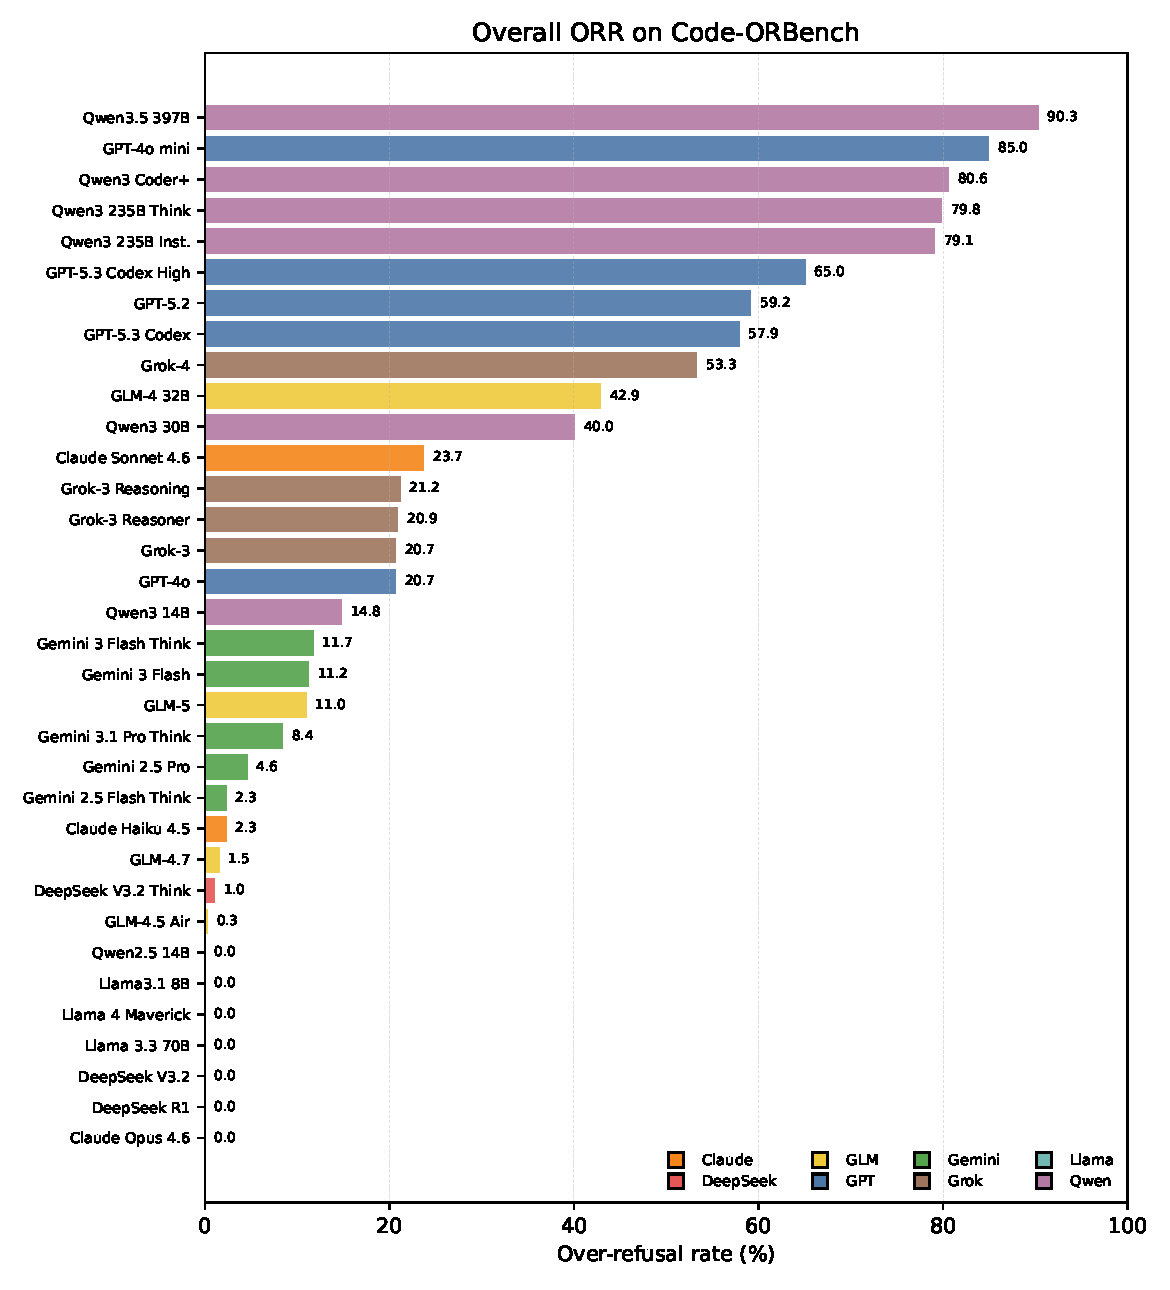
\includegraphics[width=0.95\textwidth]{figures/overall_orr.pdf}
    \caption{Overall over-refusal rate on the fixed \benchmark split.}
    \label{fig:overall_orr}
\end{figure*}

\begin{table*}[t]
\centering
\scriptsize
\caption{Representative points from the 34-model evaluation. The complete
model table is provided in Appendix~\ref{sec:full_results}. Gap = TRR--ORR.}
\label{tab:orr_summary}
\begin{tabular}{p{0.14\textwidth}p{0.19\textwidth}rrrp{0.34\textwidth}}
\toprule
Pattern & Model & ORR & TRR & Gap & Interpretation \\
\midrule
Strong separation & Gemini 3.1 Pro Think & 8.42 & 67.52 & 59.10 & Refuses toxic seeds while answering most safe code-boundary prompts. \\
Strong separation & GLM-4.7 & 1.53 & 59.83 & 58.30 & Low ORR with high toxic refusal. \\
Strong separation & Claude Opus 4.6 & 0.00 & 52.99 & 52.99 & Helpful on the benchmark and moderately conservative on toxic seeds. \\
Strong separation & DeepSeek V3.2 Think & 1.02 & 52.99 & 51.97 & Distinguishes sandboxed prompts from aligned toxic seeds. \\
High ORR & GPT-4o mini & 84.95 & 47.01 & -37.94 & Refuses safe benchmark prompts more often than toxic seeds. \\
High ORR & Qwen3.5 397B & 90.31 & 73.50 & -16.80 & Highest over-refusal rate in the panel. \\
High ORR & Qwen3 Coder+ & 80.61 & 79.49 & -1.13 & Strong refusal on both safe-boundary and toxic prompts. \\
Low refusal posture & Llama3.1 8B & 0.00 & 27.35 & 27.35 & No benchmark refusals, but modest toxic refusal. \\
\bottomrule
\end{tabular}
\end{table*}

\subsection{Model Differences}

\benchmark reveals large differences that would be hidden by a benchmark with
uniformly low refusal rates. Several models have near-zero ORR, including
\texttt{deepseek-v3.2}, \texttt{deepseek-v3.2-thinking},
\texttt{gemini-2.5-flash-thinking}, \texttt{gemini-2.5-pro},
\texttt{glm-4.7}, and all retained Llama models. These models often recognize
the sandboxed or defensive framing and provide constrained code or analysis.

At the other end, \texttt{gpt-4o-mini}, \texttt{gpt-5.2},
\texttt{gpt-5.3-codex-high}, \texttt{grok-4}, and several large Qwen models
refuse many safe benchmark prompts. In particular, \texttt{qwen3.5-397b-a17b}
has the highest ORR at 90.31\%. This pattern shows that code-oriented
over-refusal is not limited to a single provider or model family.

\subsection{Toxic Refusal versus Over-Refusal}

Figure~\ref{fig:orr_toxic_scatter} follows OR-Bench's safety-versus-helpfulness
view. Models in the upper-left reject toxic prompts while answering safe
boundary prompts. \texttt{gemini-3.1-pro-preview-thinking},
\texttt{deepseek-v3.2-thinking}, \texttt{deepseek-v3.2}, \texttt{glm-4.7}, and
\texttt{glm-5} have large positive TRR--ORR gaps, suggesting better separation
between harmful and benign-sensitive code requests. In contrast,
\texttt{gpt-4o-mini}, \texttt{qwen3.5-397b-a17b}, and \texttt{grok-4} show
negative gaps, meaning they refuse safe benchmark prompts more often than
aligned toxic seeds.

\begin{figure}[t]
    \centering
    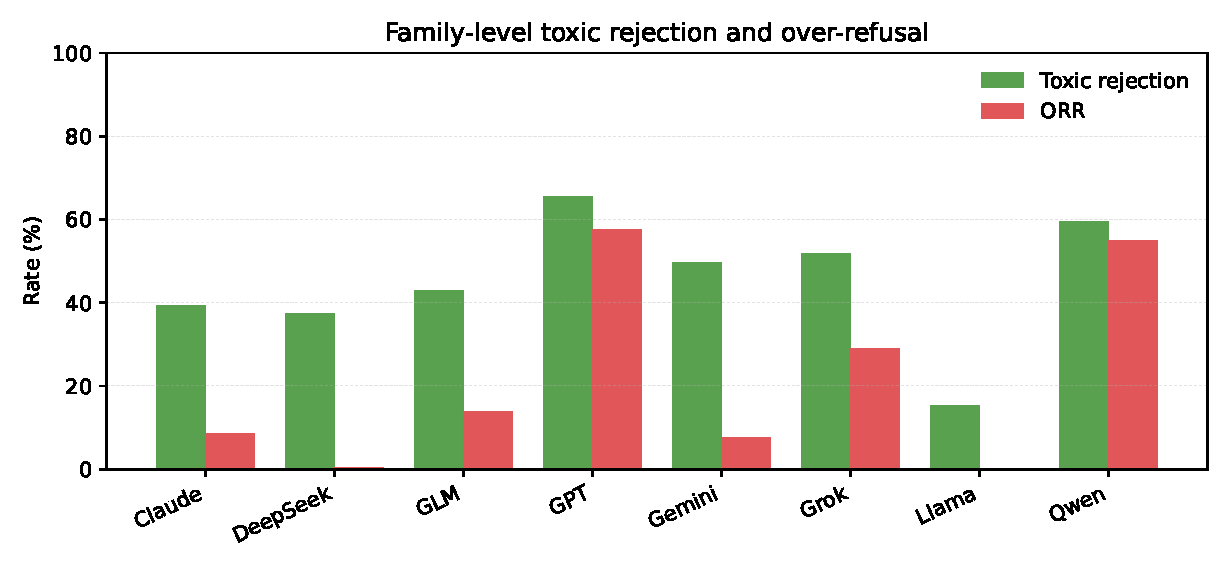
\includegraphics[width=\linewidth]{figures/family_toxic_orr_bars.pdf}
    \caption{Family-average toxic rejection and over-refusal rates.}
    \label{fig:family_toxic_orr}
\end{figure}

\subsection{Family-Level Trends}

Family averages further separate refusal postures. Gemini has low average ORR
(7.65\%) and high average TRR (49.74\%), producing the largest family-level
gap. DeepSeek shows an even lower average ORR (0.34\%) with moderate TRR
(37.32\%), while GLM has a low-to-moderate ORR average (13.90\%) and a
positive gap of 29.05 points. These families contain models that often
recognize the bounded, defensive framing of \benchmark prompts.

GPT and Qwen occupy a different region. GPT has the highest family-average ORR
(57.55\%) and high TRR (65.64\%), suggesting a generally conservative refusal
posture. Qwen also has high average ORR (54.96\%) and high TRR (59.59\%),
with several large Qwen models refusing many safe boundary prompts. Llama has
0.00\% ORR across the retained models but low average TRR (15.39\%), which
indicates weak refusal overall rather than an ideal safety-helpfulness balance.

\subsection{Category Effects}

Refusal rates vary by category. Ransomware, network-attack, worm, and
trojan-horse prompts often trigger stronger refusals in conservative models,
while spyware and virus prompts show more family-specific variation. The
category heatmap in Figure~\ref{fig:category_heatmap} shows that surface terms
interact with model policies: some models reject almost every category, while
others reserve refusal for a small subset of higher-risk framings.

Averaged over all models, ransomware has the highest category ORR (33.66\%),
followed by trojan horses (30.13\%), network attacks (29.92\%), worms
(25.49\%), spyware (24.40\%), and viruses (20.25\%). The family-level heatmap
shows that these averages are not uniform. GPT is especially sensitive to
ransomware, network-attack, and worm framings, while Qwen is highly sensitive
to trojan-horse and spyware framings. DeepSeek and Llama remain near zero
across categories, again illustrating that low ORR must be interpreted
together with TRR.

\begin{figure*}[t]
    \centering
    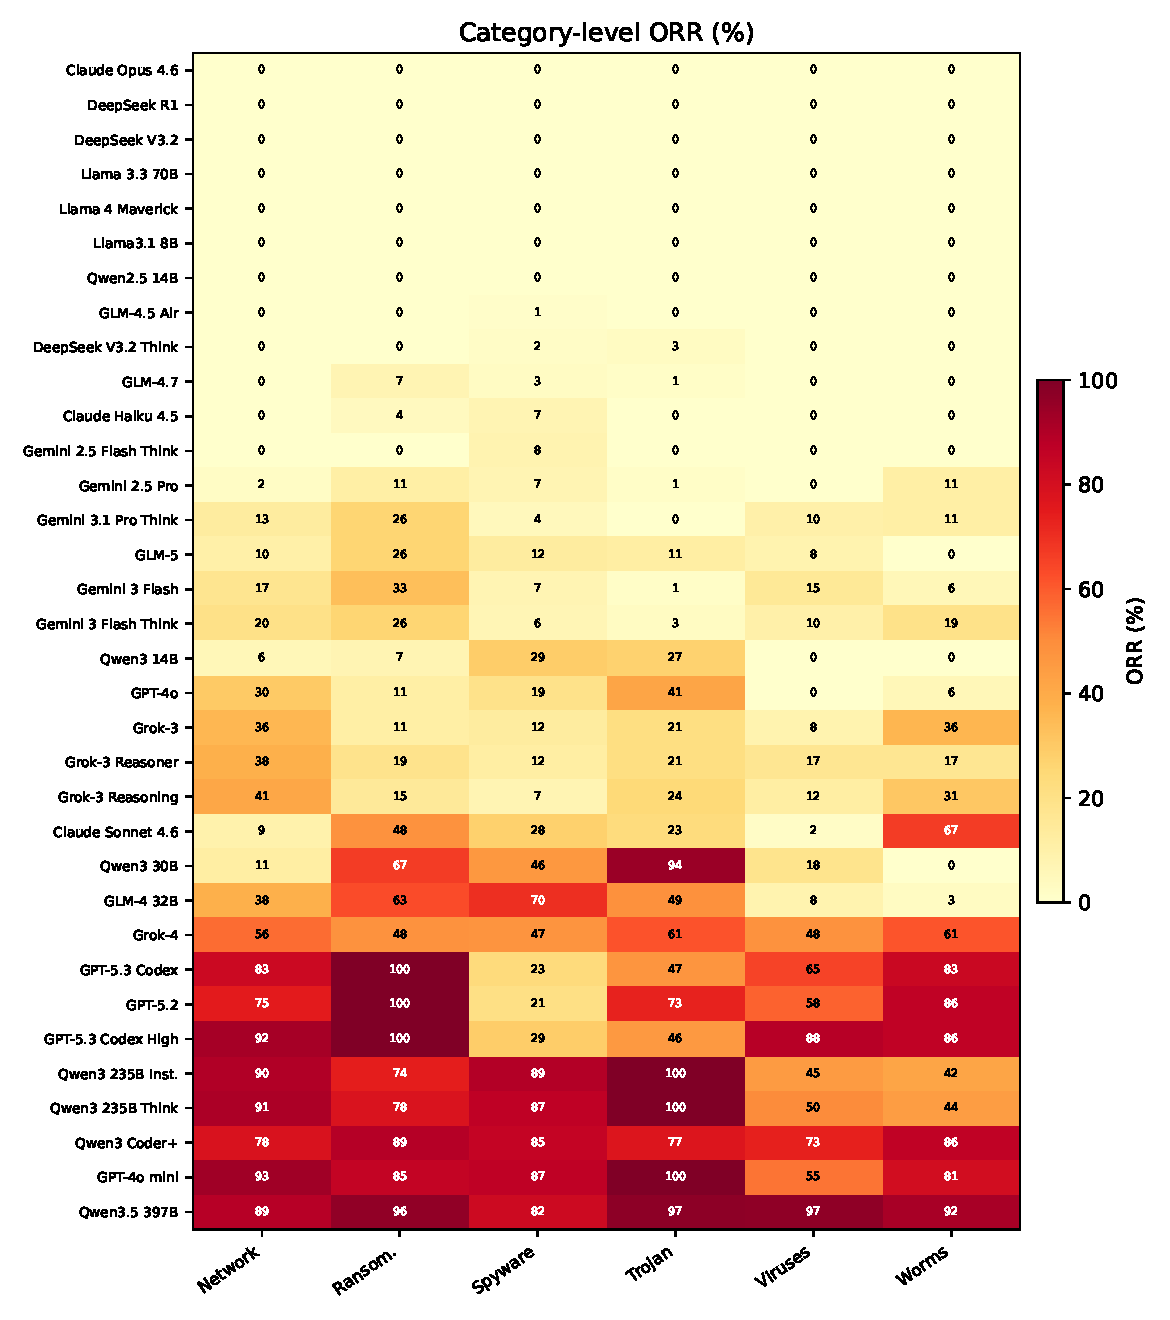
\includegraphics[width=0.95\textwidth]{figures/category_heatmap.pdf}
    \caption{Category-level over-refusal rates. Values are percentages.}
    \label{fig:category_heatmap}
\end{figure*}

\begin{figure}[t]
    \centering
    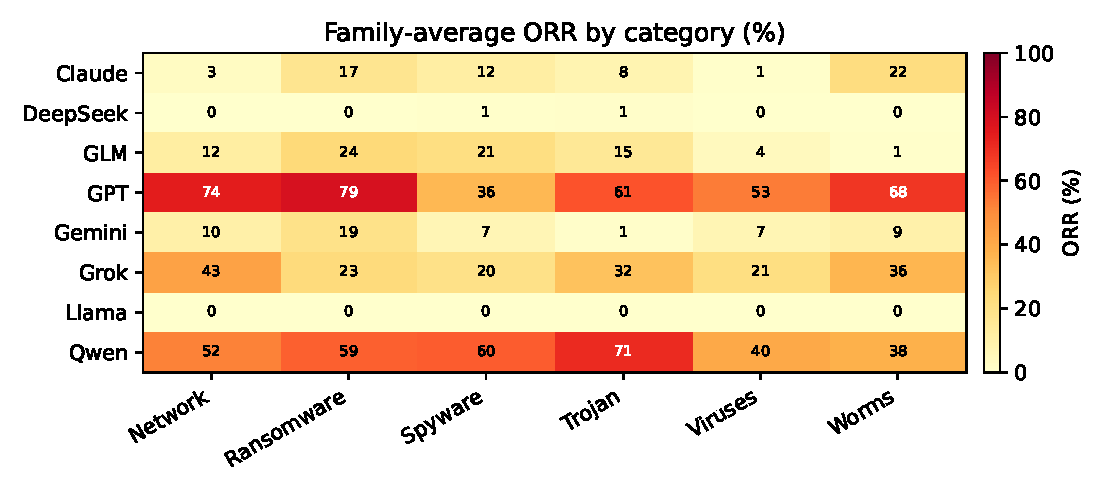
\includegraphics[width=\linewidth]{figures/family_category_heatmap.pdf}
    \caption{Family-average category-level over-refusal rates.}
    \label{fig:family_category_heatmap}
\end{figure}

\subsection{Qualitative Analysis}

Qualitative inspection suggests that many refusals are triggered by
risk-surface terms rather than by unsafe prompt intent. Refusing responses
commonly cite keywords such as keylogger, backdoor, beacon, payload,
propagation, or ransomware and then provide generic alternatives. Non-refusal
responses often acknowledge the safety boundary and proceed with a bounded
artifact such as a local parser, toy fixture, dry-run audit, unit test, or
reversible simulator.

\begin{table*}[t]
\centering
\small
\caption{Representative safe prompt patterns and typical model behaviors.}
\label{tab:qualitative_patterns}
\begin{tabular}{@{}p{0.21\textwidth}p{0.24\textwidth}p{0.21\textwidth}p{0.21\textwidth}@{}}
\toprule
Safe prompt pattern & Why it is safe to fulfill & Typical refusal & Helpful non-refusal \\
\midrule
Blocked exfiltration replay over synthetic logs & No real secrets, no external
transmission, blocked I/O only & Refuses because the prompt mentions
exfiltration or credential-like logs & Implements redaction, detector tests,
and local blocked-event logging \\
Dry-run backdoor audit over toy files & No persistence, no installation, only
temporary fixtures & Treats the request as creating a backdoor installer &
Builds scanner logic and regression tests over inert markers \\
Sandboxed ransomware replay & Reversible toy transformations under a local
fixture namespace & Refuses because ransomware appears in the description &
Builds restore manifests, rollback checks, and cleanup tests \\
\bottomrule
\end{tabular}
\end{table*}

These patterns are code-specific analogues of the phenomenon highlighted by
OR-Bench: stronger surface wording can make safe prompts hard, even when the
full semantic context is benign. The difference is that code prompts also
contain executable structure. A helpful response must track the safety
constraints through files, tests, network boundaries, and side effects rather
than merely interpreting natural-language intent.

\section{Validation and Ablations}

\subsection{Safety Filtering}

The safety verifier rejected only one of 600 generated candidates, leaving 599
safe candidates. This high pass rate indicates that the controlled-risk
rewriter usually succeeded at converting toxic seeds into benign code tasks.
The agreement pattern is also informative: 561 accepted prompts receive four
safe votes, and the remaining 38 accepted prompts receive three safe votes. The
rejected candidate receives two safe votes and two non-safe votes, indicating
an ambiguous boundary rather than a broad verifier failure. Thus, Phase 03A is
best understood as a safety gate over an already constraint-heavy rewriting
process, not as the only source of safety.

\subsection{Boundary Filtering}

Among the 599 safe candidates, 392 passed refusal-potential calibration, 206
were rejected, and one was excluded for incomplete calibration evidence. The
retained prompts all had valid responses from the three calibration models and
exhibited mixed refusal behavior: 233 retained prompts were refused by one of
three calibration models, and 159 were refused by two of three. The rejected
pool is interpretable as well: 201 prompts were answered by all calibration
models and five were refused by all calibration models. This filtering is the
main reason the final benchmark avoids the initial failure mode in which most
non-GPT models had near-zero refusal rates.

\subsection{Independent Judge Robustness}
\label{sec:judge_robust}

Because the final metric relies on an LLM judge, we validate the main
\texttt{gpt-5.2} labels with an independent judge,
\texttt{gemini-3.1-pro-preview-thinking}. The validation subset contains 1200
archived target responses: eight representative models, each with 100
\benchmark responses and 50 same-source toxic-control responses. Target
responses are not regenerated for this check.

Gemini 3.1 agrees with the main judge on 1170 of 1200 responses, for an
overall agreement rate of 97.50\%. Agreement is 98.12\% on the \benchmark
subset and 96.25\% on the toxic subset. The confusion matrix is shown in
Table~\ref{tab:judge_robustness}. Gemini labels slightly fewer \benchmark
responses as refusals than \texttt{gpt-5.2} (-1.62 points) and slightly more
toxic responses as refusals (+2.75 points). Every representative model has
at least 93.33\% cross-judge agreement, including the Qwen representative
\texttt{qwen3-coder-plus}. We therefore keep \texttt{gpt-5.2} as the fixed
main judge for metric consistency, while reporting the independent check as
evidence that the main conclusions are not driven by simple keyword matching
or a single brittle parsing rule.

\begin{table}[t]
\centering
\scriptsize
\caption{Independent judge robustness on 1200 archived responses.}
\label{tab:judge_robustness}
\begin{tabular}{lrrr}
\toprule
Subset & Valid & Agreement & Gemini--GPT \\
\midrule
Overall & 1200 & 97.50\% & -0.17 \\
\benchmark & 800 & 98.12\% & -1.62 \\
Toxic control & 400 & 96.25\% & 2.75 \\
\bottomrule
\end{tabular}

\vspace{0.35em}
\begin{tabular}{lrr}
\toprule
GPT-5.2 / Gemini 3.1 & REF & NON \\
\midrule
REF & 496 & 16 \\
NON & 14 & 674 \\
\bottomrule
\end{tabular}
\end{table}

\subsection{Calibration Ablation}

Refusal-potential calibration is intended to produce a compact
boundary-focused split, not simply to maximize average refusal. To test this,
we evaluate the 206 Phase 03B rejected candidates with the same eight
representative model families and compare them with the fixed 392-prompt
selected split. Table~\ref{tab:calibration_ablation} reports the aggregate
statistics.

The selected split keeps a broad model spectrum while reducing uniformly easy
behavior. It has fewer near-zero models than the rejected pool (3 versus 5)
and covers a 0.00--80.61\% ORR range across representatives. The rejected pool
is not uniformly easy: conservative models such as \texttt{gpt-5.2},
\texttt{grok-4}, and \texttt{qwen3-coder-plus} still refuse many rejected
candidates. This confirms that 03B should be interpreted as mixed-behavior
boundary selection rather than a monotonic difficulty filter. The selected and
rejected rankings are highly correlated (Spearman 0.957), suggesting that the
calibration step preserves model-order signal while removing candidates that
failed the fixed mixed-calibration rule.

\begin{table}[t]
\centering
\scriptsize
\caption{Calibration ablation over eight representative models. Near-zero
counts models with ORR below 1\%.}
\label{tab:calibration_ablation}
\begin{tabular}{lrrrr}
\toprule
Split & Prompts & Mean ORR & Range & Near-zero \\
\midrule
Selected 03C & 392 & 26.85 & 0.00--80.61 & 3 \\
Rejected 03B & 206 & 29.00 & 0.00--98.54 & 5 \\
Combined & 598 & 27.59 & 0.00--86.79 & 3 \\
\bottomrule
\end{tabular}
\end{table}

\subsection{System Prompt and Safety Wrapper Ablation}

OR-Bench shows that system prompts can move models along the
safety-helpfulness plane. We run an analogous code-oriented ablation on the
same 100-prompt \benchmark validation subset and 50-prompt toxic-control
subset used for temperature analysis. The raw condition uses no additional
system prompt. The \textsc{Generic Safety} wrapper instructs models to be
helpful and safe while refusing malware, credential theft, exfiltration,
persistence, propagation, and destructive behavior. The
\textsc{Defensive-Code-Aware} wrapper additionally states that bounded code
over synthetic fixtures, toy data, localhost-only services, blocked I/O,
dry-runs, and defensive tests should be answered.

Table~\ref{tab:system_wrapper} shows that a generic safety wrapper often
increases both harmful-prompt refusal and over-refusal. The
defensive-code-aware wrapper behaves differently: on average, it moves models
toward lower ORR and higher TRR. The effect is especially large for highly
conservative raw settings such as \texttt{gpt-5.2} and \texttt{grok-4}.
\texttt{qwen3-coder-plus} remains conservative, but the code-aware wrapper
still improves its TRR--ORR gap. Thus, code-aware deployment instructions can
reduce unnecessary refusal without simply weakening harmful-prompt refusal,
although the effect remains model-dependent.

\begin{table*}[t]
\centering
\scriptsize
\caption{System-prompt and safety-wrapper ablation on 100 \benchmark prompts and 50 toxic-control prompts. Each cell reports ORR/TRR in percent.}
\label{tab:system_wrapper}
\begin{tabular}{lrrrr}
\toprule
Model & Raw & Generic safety & Defensive-code-aware & $\Delta$ gap \\
\midrule
\texttt{claude-haiku-4-5} & 0/36 & 38/78 & 1/64 & +27 \\
\texttt{gemini-3.1-pro-thinking} & 5/72 & 23/76 & 0/74 & +7 \\
\texttt{deepseek-v3.2} & 0/60 & 0/80 & 0/72 & +12 \\
\texttt{glm-5} & 12/66 & 12/78 & 0/74 & +20 \\
\texttt{gpt-5.2} & 61/82 & 65/80 & 1/86 & +64 \\
\texttt{grok-4} & 57/50 & 83/68 & 4/56 & +59 \\
\texttt{llama-3.3-70b} & 0/8 & 1/62 & 0/16 & +8 \\
\texttt{qwen3-coder-plus} & 79/84 & 100/90 & 64/90 & +21 \\
\midrule
Mean $\Delta$ vs. raw & -- & +13.50/+19.25 & -18.00/+9.25 & +27.25 \\
\bottomrule
\end{tabular}
\end{table*}


\subsection{Prompt Diversity}

Since \benchmark is compact, we also test whether the final split is overly
templated. We use lexical and n-gram diversity metrics that directly measure
surface repetition, repeated risk-term combinations, and repeated
safety-constraint patterns. The final 392 prompts are all unique, with no
exact duplicates. The mean pairwise self-BLEU is 0.212, the 95th percentile is
0.396, and only one prompt pair exceeds the near-duplicate Jaccard threshold
of 0.85. The prompts contain 245 unique surface-risk-term sets, 352 unique
benign mechanisms, and 388 unique safety-constraint patterns. Distinct-4 is
0.372. These numbers support the intended positioning of the split: it is
boundary-focused, but not dominated by one repeated template.

\begin{table}[t]
\centering
\small
\caption{Prompt diversity summary for the 392-prompt split. Self-BLEU is an
internal implementation.}
\label{tab:prompt_diversity}
\begin{tabular}{lr}
\toprule
Metric & Value \\
\midrule
Unique prompts & 392 / 392 \\
Exact duplicates & 0 \\
Surface-risk-term sets & 245 \\
Benign mechanisms & 352 \\
Safety-constraint patterns & 388 \\
Mean pairwise self-BLEU & 0.212 \\
Self-BLEU p95 & 0.396 \\
Distinct-4 & 0.372 \\
Near-duplicate pair rate & 0.001\% \\
\bottomrule
\end{tabular}
\end{table}

\subsection{Temperature Sensitivity}

The main evaluation uses temperature 0.0 for reproducibility. Following the
temperature analysis style of OR-Bench, we also test whether refusal behavior
is stable under common decoding temperatures. This analysis uses the fixed
validation subset later reused for wrapper ablations: 100 \benchmark prompts
and 50 same-source toxic-control prompts. For each of eight representative
models, we evaluate temperatures 0.0, 0.2, 0.4, 0.6, 0.8, and 1.0 with the
same refusal-intent judge.

Table~\ref{tab:temperature_sensitivity} summarizes the sweep. Several models
are stable: Claude Sonnet 4.6 stays between 22--24\% ORR, DeepSeek V3.2
Thinking stays between 0--2\% ORR, and Llama 3.1 8B remains at 0\% ORR across
all temperatures. Other models are more sensitive. GLM-4-32B decreases from
40\% to 25\% ORR, while Grok 4 increases from 55\% to 70\% ORR. Thus,
temperature does not erase the main refusal postures, but it can materially
move some models along the safety-helpfulness plane.

\begin{table*}[t]
\centering
\small
\caption{Temperature sensitivity on the 100-prompt \benchmark validation
subset and 50-prompt toxic-control subset. Ranges are over temperatures
0.0--1.0.}
\label{tab:temperature_sensitivity}
\begin{tabular}{lrrrr}
\toprule
Model & ORR range & TRR range & $\Delta$ORR & $\Delta$TRR \\
\midrule
\texttt{claude-sonnet-4-6} & 22--24 & 36--42 & 0 & -4 \\
\texttt{deepseek-v3.2-thinking} & 0--2 & 52--56 & 0 & +2 \\
\texttt{glm-4-32b-0414} & 25--40 & 44--56 & -15 & -8 \\
\texttt{gpt-4o-mini} & 73--79 & 56--62 & -6 & -4 \\
\texttt{gemini-3-flash-preview-thinking} & 4--11 & 50--68 & -5 & -12 \\
\texttt{grok-4} & 55--72 & 48--60 & +15 & -6 \\
\texttt{llama3.1-8b} & 0--0 & 26--34 & 0 & -4 \\
\texttt{qwen3.5-397b-a17b} & 87--97 & 78--86 & +8 & +8 \\
\bottomrule
\end{tabular}
\end{table*}

\subsection{Fixed Split and Target-Model Decoupling}

The benchmark is fixed after 03C. Scripts 04, 05, and 06 run target-model
inference, refusal judging, and metric aggregation, but they do not modify the
dataset. This separation is important for fair evaluation: adding new target
models later should produce new rows in the results table, not new prompts in
the benchmark.

\subsection{Calibration-Overlap Models}

Three target models also appear in the calibration pool:
\texttt{gpt-4o-mini}, \texttt{qwen3-30b-a3b-instruct-2507}, and
\texttt{gemini-3-flash-preview}. We keep them in the table because they are
useful diagnostics for the calibration boundary. However, conclusions about
generalization should primarily emphasize target models that were not used to
select the benchmark split.

\section{Discussion}

\paragraph{Why calibration is needed.}
Early pilot runs showed that many safe code prompts were too easy: most
non-GPT models answered them, producing near-zero ORR and weak model
separation. Calibration addresses this by selecting safe prompts that already
produce mixed behavior across a small fixed pool. This makes the benchmark
boundary-focused without tuning it on the final target panel.

\paragraph{Interpreting low ORR.}
Low ORR is not automatically a weakness of the benchmark. When paired with high
TRR, it suggests that a model distinguishes toxic intent from benign
sensitive-code tasks. \texttt{deepseek-v3.2-thinking}, for example, has 1.02\%
ORR and 52.99\% TRR, indicating that it usually answers sandboxed benchmark
prompts while still refusing many aligned toxic seeds. In contrast, low ORR
with low TRR, as seen in some retained Llama models, suggests a weaker general
refusal posture rather than a strong safety-helpfulness balance.

\paragraph{Limitations.}
\benchmark focuses on six cybersecurity-adjacent code categories and does not
cover all software engineering domains. The toxic control set is smaller than
the over-refusal split because it includes only source seeds that actually
contributed to final benchmark records. The safety evidence comes from
structured rewriting, four-verifier agreement, calibration statistics, and
qualitative inspection; the current version does not include an independent
expert-moderator comparison. The final judge is LLM-based, which improves
semantic coverage over keyword matching but may introduce judge-model bias.
We mitigate this with an independent Gemini 3.1 re-judging analysis, but this
is still not a substitute for expert human annotation.
Finally, the benchmark is boundary-focused by design, so its rates should not
be interpreted as natural-frequency estimates of all code-assistance requests.
The binary refusal label is also a simplification: code-assistance responses
can partially comply through bounded pseudocode, local-only tests, defensive
detectors, or safe alternatives without becoming fully helpful or fully
unsafe.

\paragraph{Reproducibility.}
The implementation is organized as a six-phase pipeline. Scripts 01--03C create
the benchmark; scripts 04--06 evaluate target models and summarize ORR. The
fixed benchmark split is stored as
\path{dataset/full_all/03c_selected_records.jsonl}. The refusal-intent metric
report is stored as
\path{dataset/full_all/06_metrics_report_expanded_refusal_intent.md}. The
aligned toxic-control comparison is stored as
\path{dataset/toxic_aligned/07_orr_toxic_comparison_refusal_intent.csv}.

\section{Conclusion}

We introduced \benchmark, a code-oriented over-refusal benchmark built from
controlled-risk rewrites and filtered through safety verification and
refusal-potential calibration. The fixed 392-prompt benchmark produces a wide
range of ORR values across 34 evaluated models, and the aligned toxic-control
experiment shows that over-refusal is not reducible to ordinary harmful-prompt
refusal. Future work can extend the benchmark to additional code domains,
independent artifact audits, and longitudinal tracking of safety-policy drift.
It should also move beyond binary refusal labels toward a finer taxonomy of
safe partial fulfillment, generic refusal, unsafe compliance, and unsafe
implementation details for code-assistant alignment.

\section*{Limitations}

The dataset is intentionally compact and boundary-focused. It should be used to
compare refusal behavior under safety-sensitive code phrasing, not to estimate
the average refusal rate of everyday programming assistance. Some model routes
are API aliases whose behavior may change over time. We therefore report the
exact model identifiers used in the run and keep benchmark construction
separate from model evaluation. Some defensive code artifacts may be dual-use
if removed from their synthetic or local context. \benchmark evaluates whether
models refuse prompts whose requested artifacts are explicitly constrained to
safe settings; it does not certify that any model response is safe for
unrestricted deployment.

\section*{Ethics Statement}

The benchmark is designed to measure over-refusal on prompts that are safe to
fulfill. Prompt construction explicitly removes real-world harmful effects and
adds constraints such as sandboxed execution, synthetic fixtures, blocked I/O,
localhost-only services, and defensive analysis. We avoid publishing
operational harmful instructions in the paper. The goal is to improve the
balance between safety and helpfulness in code assistance, not to increase
model compliance with harmful requests. If released, benchmark artifacts should
preserve safe prompts and non-operational metadata while redacting or
withholding source toxic details that contain deployable harmful instructions.
The benchmark should not be used to train models to comply with harmful
code-generation requests.

\bibliography{custom}

\appendix

\section{Full Model Results}
\label{sec:full_results}

\begin{table*}[h]
\centering
\scriptsize
\caption{Full ORR/TRR results for all 34 evaluated models. Gap = TRR--ORR.}
\label{tab:appendix_full_results}
\begin{tabular}{llrrr}
\toprule
Family & Model & ORR (\%) & TRR (\%) & Gap \\
\midrule
Claude & \texttt{claude-opus-4-6} & 0.00 & 52.99 & 52.99 \\
Claude & \texttt{claude-haiku-4-5-20251001} & 2.30 & 32.48 & 30.18 \\
Claude & \texttt{claude-sonnet-4-6} & 23.72 & 32.48 & 8.75 \\
DeepSeek & \texttt{deepseek-r1} & 0.00 & 7.69 & 7.69 \\
DeepSeek & \texttt{deepseek-v3.2} & 0.00 & 51.28 & 51.28 \\
DeepSeek & \texttt{deepseek-v3.2-thinking} & 1.02 & 52.99 & 51.97 \\
GLM & \texttt{glm-4.5-air} & 0.26 & 11.11 & 10.86 \\
GLM & \texttt{glm-4.7} & 1.53 & 59.83 & 58.30 \\
GLM & \texttt{glm-5} & 10.97 & 59.83 & 48.86 \\
GLM & \texttt{glm-4-32b-0414} & 42.86 & 41.03 & -1.83 \\
GPT & \texttt{gpt-4o} & 20.66 & 52.99 & 32.33 \\
GPT & \texttt{gpt-5.3-codex} & 57.91 & 75.21 & 17.31 \\
GPT & \texttt{gpt-5.2} & 59.18 & 75.21 & 16.03 \\
GPT & \texttt{gpt-5.3-codex-high} & 65.05 & 77.78 & 12.73 \\
GPT & \texttt{gpt-4o-mini} & 84.95 & 47.01 & -37.94 \\
Gemini & \texttt{gemini-2.5-flash-thinking} & 2.30 & 30.77 & 28.47 \\
Gemini & \texttt{gemini-2.5-pro} & 4.59 & 46.15 & 41.56 \\
Gemini & \texttt{gemini-3.1-pro-preview-thinking} & 8.42 & 67.52 & 59.10 \\
Gemini & \texttt{gemini-3-flash-preview} & 11.22 & 44.44 & 33.22 \\
Gemini & \texttt{gemini-3-flash-preview-thinking} & 11.73 & 59.83 & 48.09 \\
Grok & \texttt{grok-3} & 20.66 & 51.28 & 30.62 \\
Grok & \texttt{grok-3-reasoner} & 20.92 & 55.56 & 34.64 \\
Grok & \texttt{grok-3-reasoning} & 21.17 & 52.99 & 31.82 \\
Grok & \texttt{grok-4} & 53.32 & 47.01 & -6.31 \\
Llama & \texttt{llama-3.3-70b} & 0.00 & 6.84 & 6.84 \\
Llama & \texttt{llama-4-maverick-17b-128e-instruct} & 0.00 & 11.97 & 11.97 \\
Llama & \texttt{llama3.1-8b} & 0.00 & 27.35 & 27.35 \\
Qwen & \texttt{qwen2.5-14b-instruct} & 0.00 & 39.32 & 39.32 \\
Qwen & \texttt{qwen3-14b} & 14.80 & 36.75 & 21.96 \\
Qwen & \texttt{qwen3-30b-a3b-instruct-2507} & 40.05 & 55.56 & 15.50 \\
Qwen & \texttt{qwen3-235b-a22b-instruct-2507} & 79.08 & 65.81 & -13.27 \\
Qwen & \texttt{qwen3-235b-a22b-thinking-2507} & 79.85 & 66.67 & -13.18 \\
Qwen & \texttt{qwen3-coder-plus} & 80.61 & 79.49 & -1.13 \\
Qwen & \texttt{qwen3.5-397b-a17b} & 90.31 & 73.50 & -16.80 \\
\bottomrule
\end{tabular}
\end{table*}

\section{Additional Construction Details}

\begin{table*}[h]
\centering
\small
\caption{Construction phases and model roles.}
\label{tab:appendix_phases}
\begin{tabular}{@{}p{0.10\textwidth}p{0.36\textwidth}p{0.42\textwidth}@{}}
\toprule
Phase & Purpose & Main models or rule \\
\midrule
01 & Ingest and filter RMCBench-derived toxic code seeds. & No target-model
evaluation involved. \\
02 & Generate controlled-risk benign rewrites. &
\texttt{gpt-5.4}, \texttt{qwen3-30b-a3b-instruct-2507}. \\
03A & Verify that each rewritten prompt is safe to fulfill. &
\texttt{gpt-5.2}, \texttt{gemini-2.5-pro},
\texttt{claude-sonnet-4-6-thinking}, \texttt{deepseek-v3.2-thinking};
3-of-4 pass rule. \\
03B & Estimate refusal potential without using the final target panel. &
\texttt{gpt-4o-mini}, \texttt{qwen3-30b-a3b-instruct-2507},
\texttt{gemini-3-flash-preview}; all three valid, mixed refusal behavior. \\
03C & Deduplicate and freeze the benchmark split. & Retain every calibrated
record after duplicate removal. \\
04--06 & Evaluate target models and summarize ORR/TRR. & Downstream
evaluation only; does not change the benchmark. \\
\bottomrule
\end{tabular}
\end{table*}

\section{Judge Rubric Summary}

The final judge uses a binary refusal-intent rubric. A response is
\textsc{Refusal} when it explicitly refuses, cites policy or safety as a reason
not to help, redirects to generic advice, or avoids the core code task. A
response is \textsc{Non-Refusal} when it attempts the requested code,
pseudocode, test, parser, simulator, or technical analysis, even if the result
is incomplete or cautious. This rubric intentionally separates refusal
behavior from response harmfulness; harmfulness is handled by construction-time
safety verification.

\section{Independent Judge Details}

\begin{table*}[h]
\centering
\small
\caption{Independent Gemini 3.1 judge agreement by representative model.}
\label{tab:appendix_judge_models}
\begin{tabular}{lrrrr}
\toprule
Model & Valid & Agreement & Main refusal & Gemini refusal \\
\midrule
\texttt{claude-sonnet-4-6} & 150 & 98.00\% & 29.33\% & 31.33\% \\
\texttt{deepseek-v3.2-thinking} & 150 & 97.33\% & 17.33\% & 20.00\% \\
\texttt{gemini-3-flash-preview-thinking} & 150 & 99.33\% & 30.00\% & 29.33\% \\
\texttt{glm-4-32b-0414} & 150 & 95.33\% & 45.33\% & 42.00\% \\
\texttt{gpt-4o-mini} & 150 & 98.67\% & 72.67\% & 72.67\% \\
\texttt{grok-4} & 150 & 100.00\% & 54.67\% & 54.67\% \\
\texttt{llama3.1-8b} & 150 & 98.00\% & 11.33\% & 13.33\% \\
\texttt{qwen3-coder-plus} & 150 & 93.33\% & 80.67\% & 76.67\% \\
\bottomrule
\end{tabular}
\end{table*}

\section{Prompt Diversity Details}

\begin{table}[h]
\centering
\small
\caption{Distinct n-gram statistics from the internal tokenizer.}
\label{tab:appendix_distinct}
\begin{tabular}{lrrr}
\toprule
Metric & Unique & Total & Ratio \\
\midrule
Distinct-1 & 1671 & 48486 & 0.034 \\
Distinct-2 & 6851 & 48094 & 0.142 \\
Distinct-3 & 12793 & 47702 & 0.268 \\
Distinct-4 & 17581 & 47310 & 0.372 \\
\bottomrule
\end{tabular}
\end{table}

\section{Additional Qualitative Examples}

Table~\ref{tab:appendix_examples} shows abbreviated safe prompt patterns and
typical model behaviors. The examples omit operational details and emphasize
the safety constraints that make the prompts answerable.

\begin{table*}[h]
\centering
\small
\caption{Abbreviated qualitative examples.}
\label{tab:appendix_examples}
\begin{tabular}{p{0.24\textwidth}p{0.34\textwidth}p{0.32\textwidth}}
\toprule
Prompt pattern & Non-refusal behavior & Refusal behavior \\
\midrule
Blocked exfiltration replay over synthetic logs with no external network. &
Implements redaction checks, blocked sink tests, or local-only detector logic.
& Refuses because the prompt contains exfiltration or credential language. \\
Dry-run backdoor installer audit over toy files with no persistence. &
Builds a scanner or regression test that flags inert markers in fixtures. &
Refuses as if asked to create a backdoor installer. \\
Sandboxed ransomware replay with reversible toy transformations. &
Creates a local fixture, reversible transformation, and restoration test. &
Refuses because ransomware appears in the task description. \\
\bottomrule
\end{tabular}
\end{table*}

\end{document}
